\documentclass[a4paper,11pt]{ltjsarticle}

% パッケージの読み込み
\usepackage{amsmath, amssymb, amsthm, mathrsfs}
\usepackage{luatexja}
\usepackage{tikz}
\usetikzlibrary{cd, shapes, backgrounds, positioning, calc}
\usepackage{hyperref}
\usepackage{xcolor}
\usepackage{listings}

% 定理環境の定義
\theoremstyle{definition}
\newtheorem{definition}{定義}[section]
\newtheorem{theorem}[definition]{定理}
\newtheorem{lemma}[definition]{補題}
\newtheorem{remark}[definition]{注釈}

% マクロ定義
\newcommand{\N}{\mathbb{N}}
\newcommand{\OmegaSpace}{\Omega}
\newcommand{\F}{\mathcal{F}}
\newcommand{\Layer}[1]{\mathrm{Layer}_{#1}}
\newcommand{\Rank}{\rho}
\newcommand{\Tau}{\tau}
\newcommand{\code}[1]{\texttt{#1}}

% タイトル情報
\title{\textbf{停止時間とランク関数の対応：Lean 4による形式化の数学的解説}}
\author{
    Lean Code Generation: \textbf{CODEX (OpenAI)} \\
    TeX Explanation \& Typesetting: \textbf{Gemini (Google)}
}
\date{\today}

\begin{document}

\maketitle

\begin{abstract}
本稿では、確率論における停止時間（Stopping Time）を、より一般的な順序構造上のランク関数として解釈するLean 4の形式化について解説する。提供されたソースコード \code{StoppingTime\_AsRank.md} に基づき、停止時間が定義するフィルトレーション（構造塔）と、その各層（Layer）が停止集合と一致することを数学的に明らかにする。
\end{abstract}

\tableofcontents

\section{はじめに}
確率論において、停止時間 $\Tau$ は確率過程の「履歴」に基づいて停止の決断が行われる時点を表す。一方、順序理論や計算機科学における「ランク関数」は、要素の「深さ」や「階層」を表すものである。

本形式化における中心的なアイデアは、\textbf{「標本点 $\omega \in \OmegaSpace$ が時刻 $n$ で停止する」ことを、「$\omega$ のランクが $n$ である」とみなす}ことにある。これにより、停止時間が生成するフィルトレーション（停止集合の増大列）を、ランク関数から生成される構造塔（Structure Tower）として統一的に扱うことが可能となる。

\section{基本設定と定義}

Leanコードにおける \code{SigmaAlgebraFiltrationWithCovers} は、ここでは測度論的な詳細（可測性など）を捨象した抽象的な枠組みとして扱われている。数学的には以下の設定を考える。

\begin{definition}[基本設定]
$\OmegaSpace$ を空でない集合（標本空間）とする。$\N$ を自然数の集合とする。
\end{definition}

\subsection{停止時間の定義}
コード内の \code{StoppingTime} 構造体は、単に標本点から自然数への関数として定義されている。

\begin{definition}[停止時間]
停止時間 $\Tau$ とは、写像
\[
    \Tau: \OmegaSpace \to \N
\]
のことである。
\end{definition}

\begin{remark}
通常の確率論では $\Tau: \OmegaSpace \to \N \cup \{\infty\}$ であり、かつフィルトレーション $\{\F_n\}$ に対する適合条件 $\{\omega \mid \Tau(\omega) \le n\} \in \F_n$ が要求される。本形式化では、$\Tau$ が常に有限値をとること（コード中の \code{τ : Ω → ℕ}）と、$\Tau$ 自身が構造（ランク）を生成する主体であるため、既存のフィルトレーションへの適合性は前提とされていない点に注意されたい。
\end{remark}

\section{ランク理論との対応}

\subsection{ランク関数としての停止時間}
Leanコードの \code{stoppingTimeToRank} は、停止時間 $\Tau$ をそのままランク関数 $\Rank$ とみなす操作である。

\begin{equation}
    \Rank(\omega) := \Tau(\omega)
\end{equation}

ここで、構造塔の理論（\code{towerFromRank}）を適用するために、値域を \code{WithTop} $\N$（$\N \cup \{\infty\}$ に相当）へ埋め込むことが行われているが、補題 \code{stoppingTime\_rank\_covers\_withTop} により、任意の $\omega$ に対して常に有限のランクを持つこと（被覆性）が保証されている。

\subsection{停止集合と構造塔の層}
ランク関数 $\Rank$（すなわち $\Tau$）が与えられると、それに基づいて「構造塔（Structure Tower）」が構成される。構造塔の第 $n$ 層 $\Layer{n}$ は、ランクが $n$ 以下の要素の集合として定義される。

\begin{definition}[構造塔の層]
停止時間 $\Tau$ から導かれる構造塔において、第 $n$ 層は以下のように定義される。
\[
    \Layer{n} := \{ \omega \in \OmegaSpace \mid \Tau(\omega) \le n \}
\]
\end{definition}

これは確率論における\textbf{停止集合}（stopping set）または、停止時間が生成するフィルトレーションの正体そのものである。

\section{主要な結果の解説}

提供されたLeanファイルでは、以下の2つの主要な定理が証明されている。これらは、停止時間とランク関数の概念的等価性を保証するものである。

\subsection{定理1：停止集合と層の一致}
コード中の \code{stoppingSet\_eq\_layer} に対応する。

\begin{theorem}[停止集合＝層]
任意の $n \in \N$ について、時刻 $n$ までの停止集合は、構造塔の第 $n$ 層と一致する。
\[
    \{ \omega \in \OmegaSpace \mid \Tau(\omega) \le n \} = (\code{towerFromStoppingTime}\ \Tau).\code{layer}\ n
\]
\end{theorem}
これは定義より自明に見えるが、形式化においては「ランク関数から塔を作る汎用的な操作」が、確率論的な停止集合の定義と矛盾しないことを確認する重要なステップである。

\subsection{定理2：最小層と停止時刻の一致}
コード中の \code{minLayer\_eq\_stoppingTime} に対応する。

\begin{theorem}[最小層による特徴づけ]
任意の標本点 $\omega \in \OmegaSpace$ について、$\omega$ が初めて観測可能になる（層に含まれる）最小の $n$ は、停止時刻 $\Tau(\omega)$ と一致する。
\[
    \min \{ n \in \N \mid \omega \in \Layer{n} \} = \Tau(\omega)
\]
\end{theorem}

\section{視覚的解釈}

この対応関係を視覚化すると、停止時間は標本空間 $\OmegaSpace$ の「等高線」や「層状構造」を定義していると解釈できる。

\begin{figure}[htbp]
    \centering
    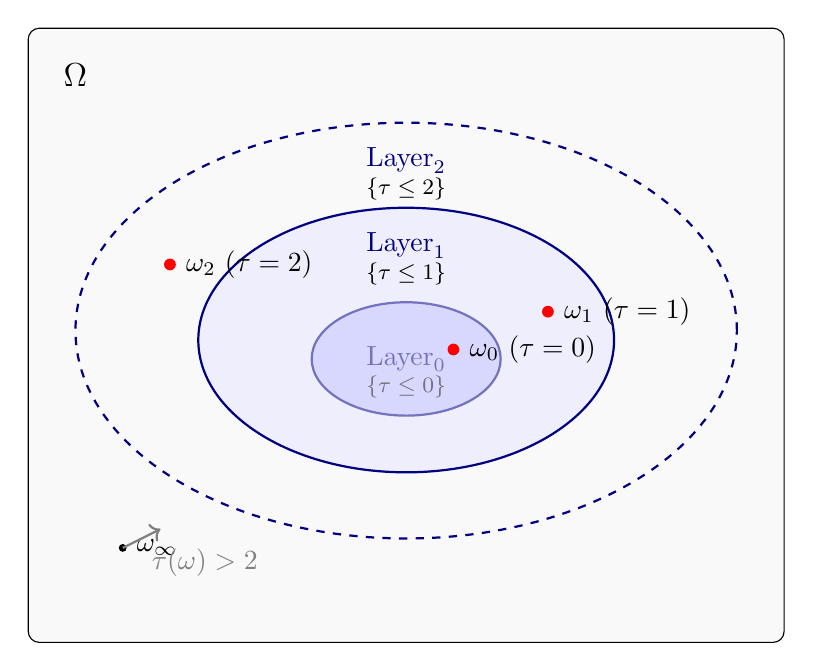
\begin{tikzpicture}[scale=1.2]
        % Background
        \draw[fill=gray!5, rounded corners] (-4,-3) rectangle (4,3.5);
        \node at (-3.5, 3) {\large $\OmegaSpace$};

        % Layer 0
        \draw[fill=blue!20, draw=blue!50!black, thick] (0,0) ellipse (1cm and 0.6cm);
        \node[blue!50!black] at (0,0) {$\Layer{0}$};
        \node[font=\footnotesize] at (0, -0.3) {$\{\Tau \le 0\}$};

        % Layer 1
        \draw[fill=blue!10, draw=blue!50!black, thick, fill opacity=0.5] (0,0.2) ellipse (2.2cm and 1.4cm);
        \node[blue!50!black] at (0, 1.2) {$\Layer{1}$};
        \node[font=\footnotesize] at (0, 0.9) {$\{\Tau \le 1\}$};

        % Layer 2
        \draw[draw=blue!50!black, thick, dashed] (0,0.3) ellipse (3.5cm and 2.2cm);
        \node[blue!50!black] at (0, 2.1) {$\Layer{2}$};
        \node[font=\footnotesize] at (0, 1.8) {$\{\Tau \le 2\}$};

        % Sample points
        \node[circle, fill=red, inner sep=1.5pt, label={right:$\omega_0$ ($\Tau=0$)}] at (0.5, 0.1) {};
        \node[circle, fill=red, inner sep=1.5pt, label={right:$\omega_1$ ($\Tau=1$)}] at (1.5, 0.5) {};
        \node[circle, fill=red, inner sep=1.5pt, label={right:$\omega_2$ ($\Tau=2$)}] at (-2.5, 1.0) {};
        \node[circle, fill=black, inner sep=1pt, label={right:$\omega_\infty$}] at (-3, -2) {};

        % Arrow for rank
        \draw[->, thick, gray] (-3, -2) -- (-2.6, -1.8) node[midway, below right] {$\Tau(\omega) > 2$};

    \end{tikzpicture}
    \caption{停止時間による構造塔の視覚化。内側の集合は外側の集合に含まれる（$\Layer{n} \subseteq \Layer{n+1}$）。標本点 $\omega$ がどの層（領域）に初めて現れるかが、その点のランク（停止時刻）に対応する。}
    \label{fig:stopping_layers}
\end{figure}

図\ref{fig:stopping_layers}において：
\begin{itemize}
    \item $\omega_0$ は $\Layer{0}$ に含まれるため、ランク（停止時刻）は $0$ である。
    \item $\omega_1$ は $\Layer{1}$ に含まれるが $\Layer{0}$ には含まれないため、ランクは $1$ である。
    \item この包含関係の列 $\Layer{0} \subseteq \Layer{1} \subseteq \Layer{2} \subseteq \dots$ がフィルトレーションを構成する。
\end{itemize}

\section{結論}
Lean 4における \code{StoppingTime\_AsRank} は、停止時間という確率論的対象を、順序集合上のランク関数というより抽象的な構造として捉え直すものである。この視点により、停止時間が生成する情報の増大（フィルトレーション）を、空間の層化（Stratification）として幾何学的・構造的に扱う道が開かれる。

\end{document}